En esta sección se compararon las distintas heuristicas implementadas en el trabajo. Por un lado, la heuristica golosa y por otro la heuristica de busqueda local.\\
Dada la naturaleza del problema, no existe un único factor a analizar como en trabajos anteriores en los que solo interesaba el tiempo de corrida. Sino que también, al ser un problema de optimización, entra en juego la calidad de las soluciones. \\

\subsection{Calidad de solución}
Primero analizaremos la calidad de las soluciones obtenidas por las heuristicas. Para realizar este analisis se implementó un generador de grafos aleatorios y en base a estos se corrieron los distintos algoritmos. \\
Estos experimentos se dividieron en dos etapas, uno que intenta medir la calidad de soluciones en grafos donde resulta posible su coloreo total y otro que toma en cuenta cualquier tipo de grafo.\\

Para medir la calidad de soluciones, consideramos el porcentaje de aristas sin conflictos (con ambos extremos pintados y de distinto color) sobre el total de aristas del grafo.

\subsubsection{Grafos coloreables}

Para realizar este experimento, se utilizó el generador de grafos aleatorios y se filtro a cada uno por los que el algoritmo del ejercicio 2 indicaba que eran coloreables. \\

Debido a la lentitud de este metodo, no se obtuvo un conjunto de grafos muy grande. \\

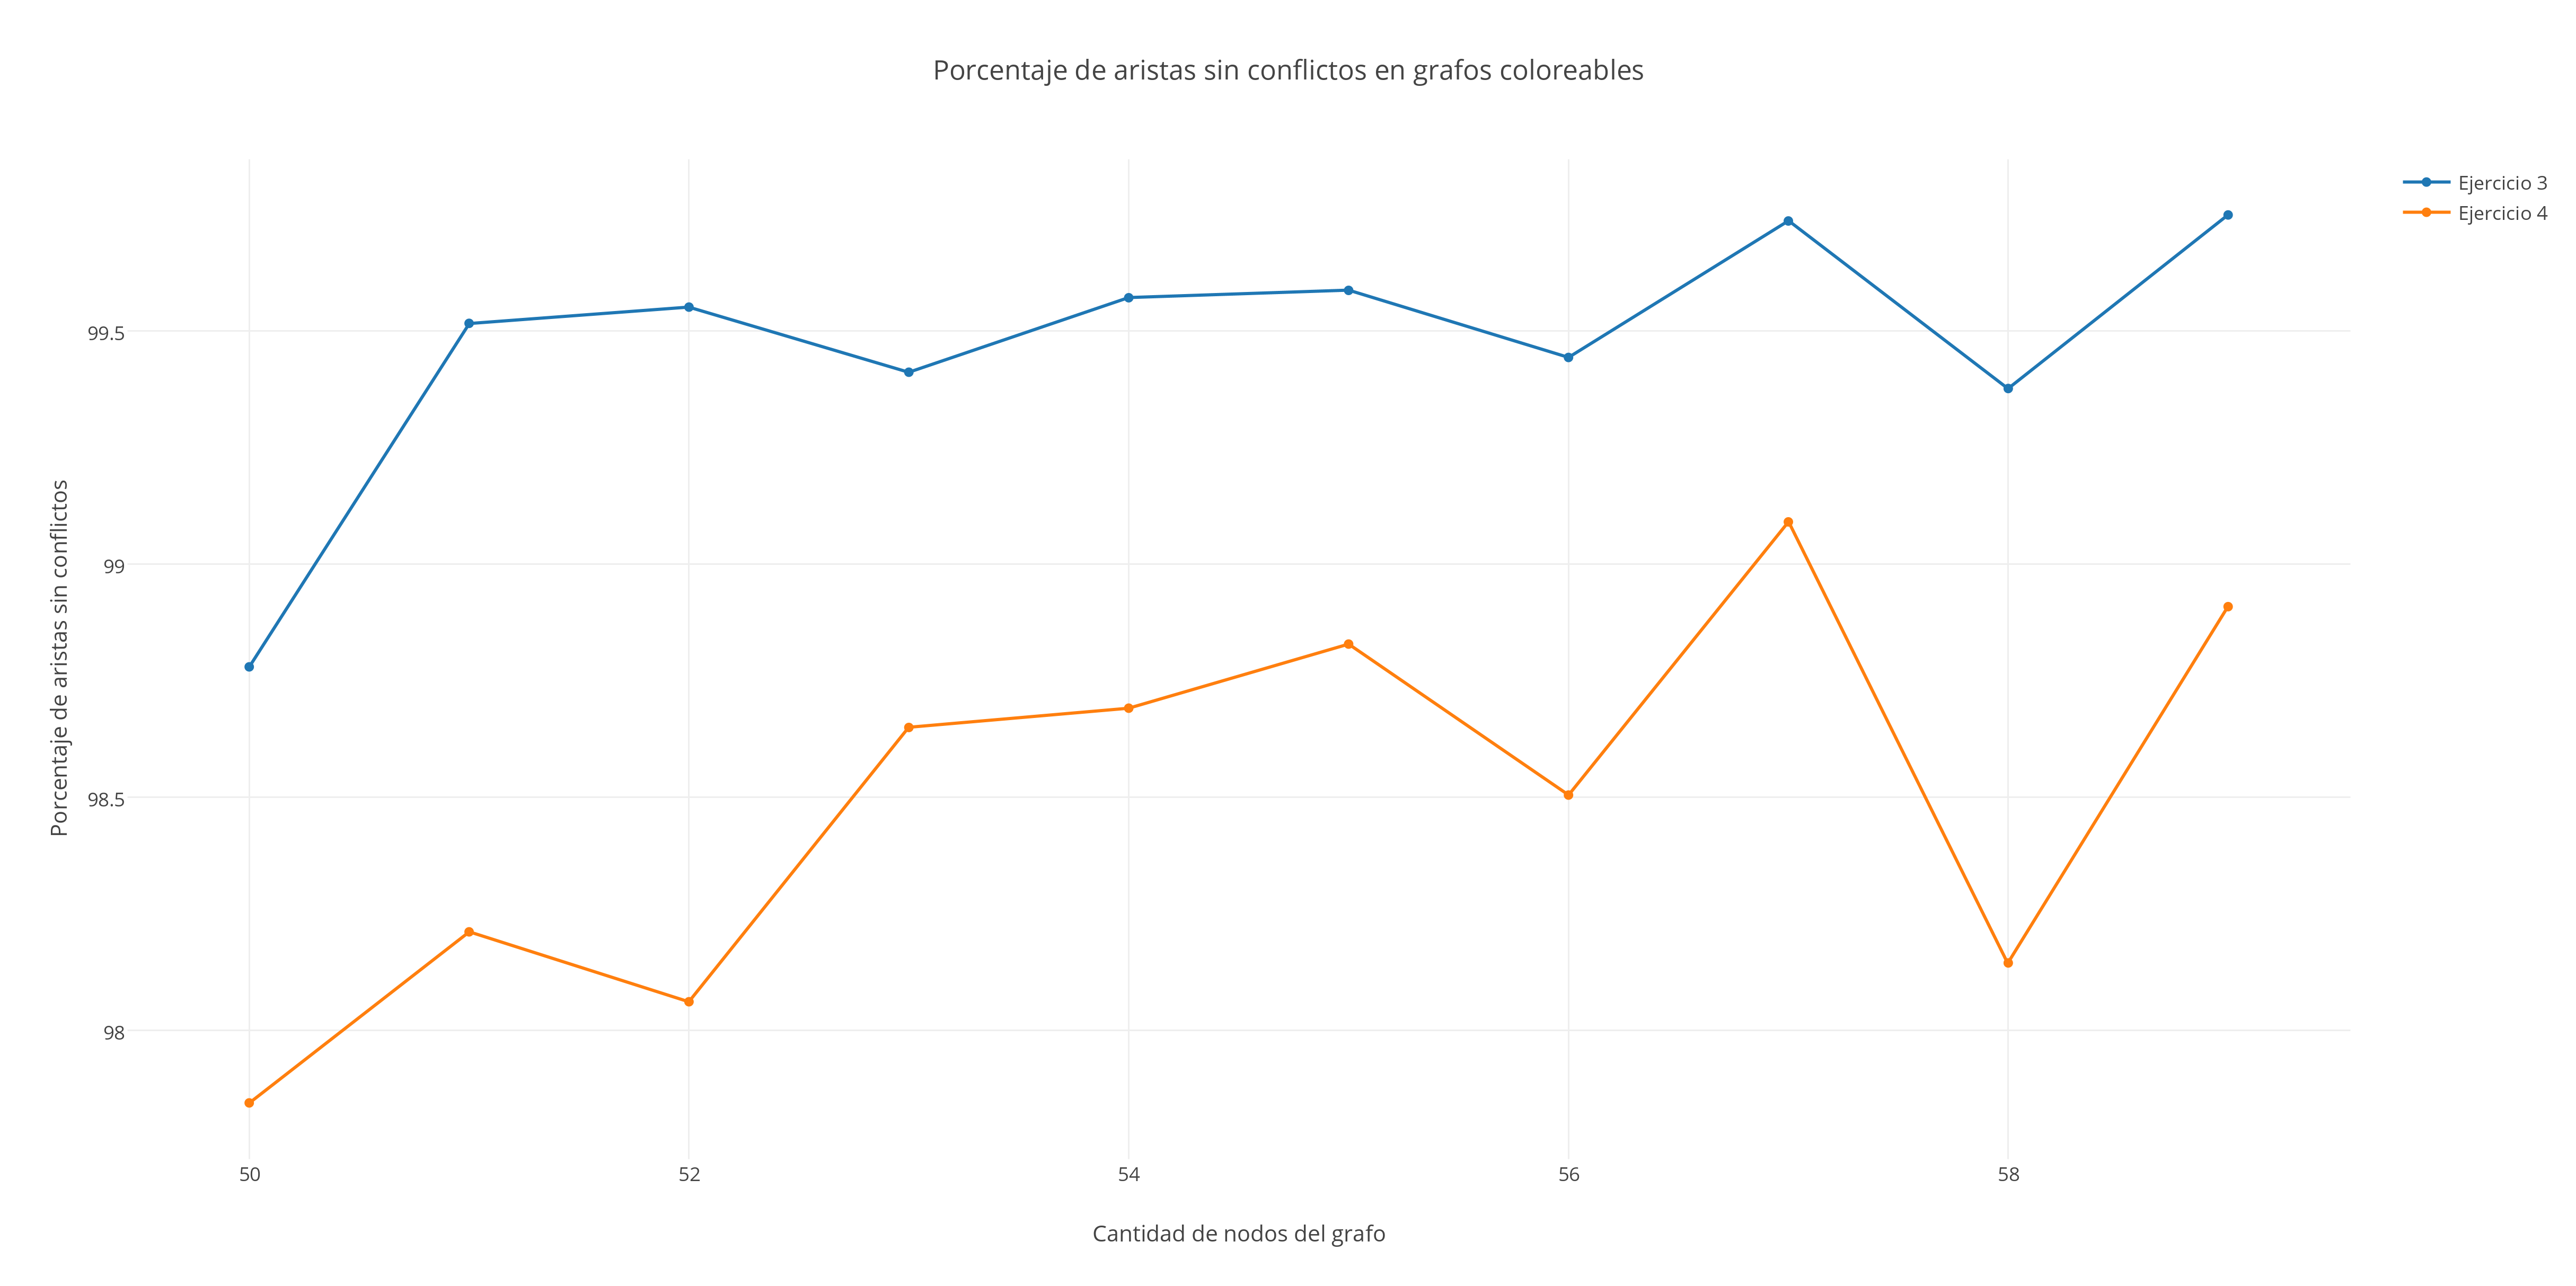
\includegraphics[scale=0.45]{./imagenes5/coloreables.png}
 	{}

En el gráfico anterior se puede notar, que si bien la heuristica del ejercicio 3 presenta soluciones mas cercanas para este conjunto de grafos, ambas están muy cercanas a la solución optima.


\subsubsection{Grafos no necesariamente coloreables}

En estos experimentos, tomamos grafos aleatorios variando tamaño y cantidad de colores. Se comparó la calidad de las soluciones provistas por los dos algoritmos.\\

En el siguiente experimento se corrió a los dos algoritmos con grafos de distinto tamaño, pero con 2 colores en total.
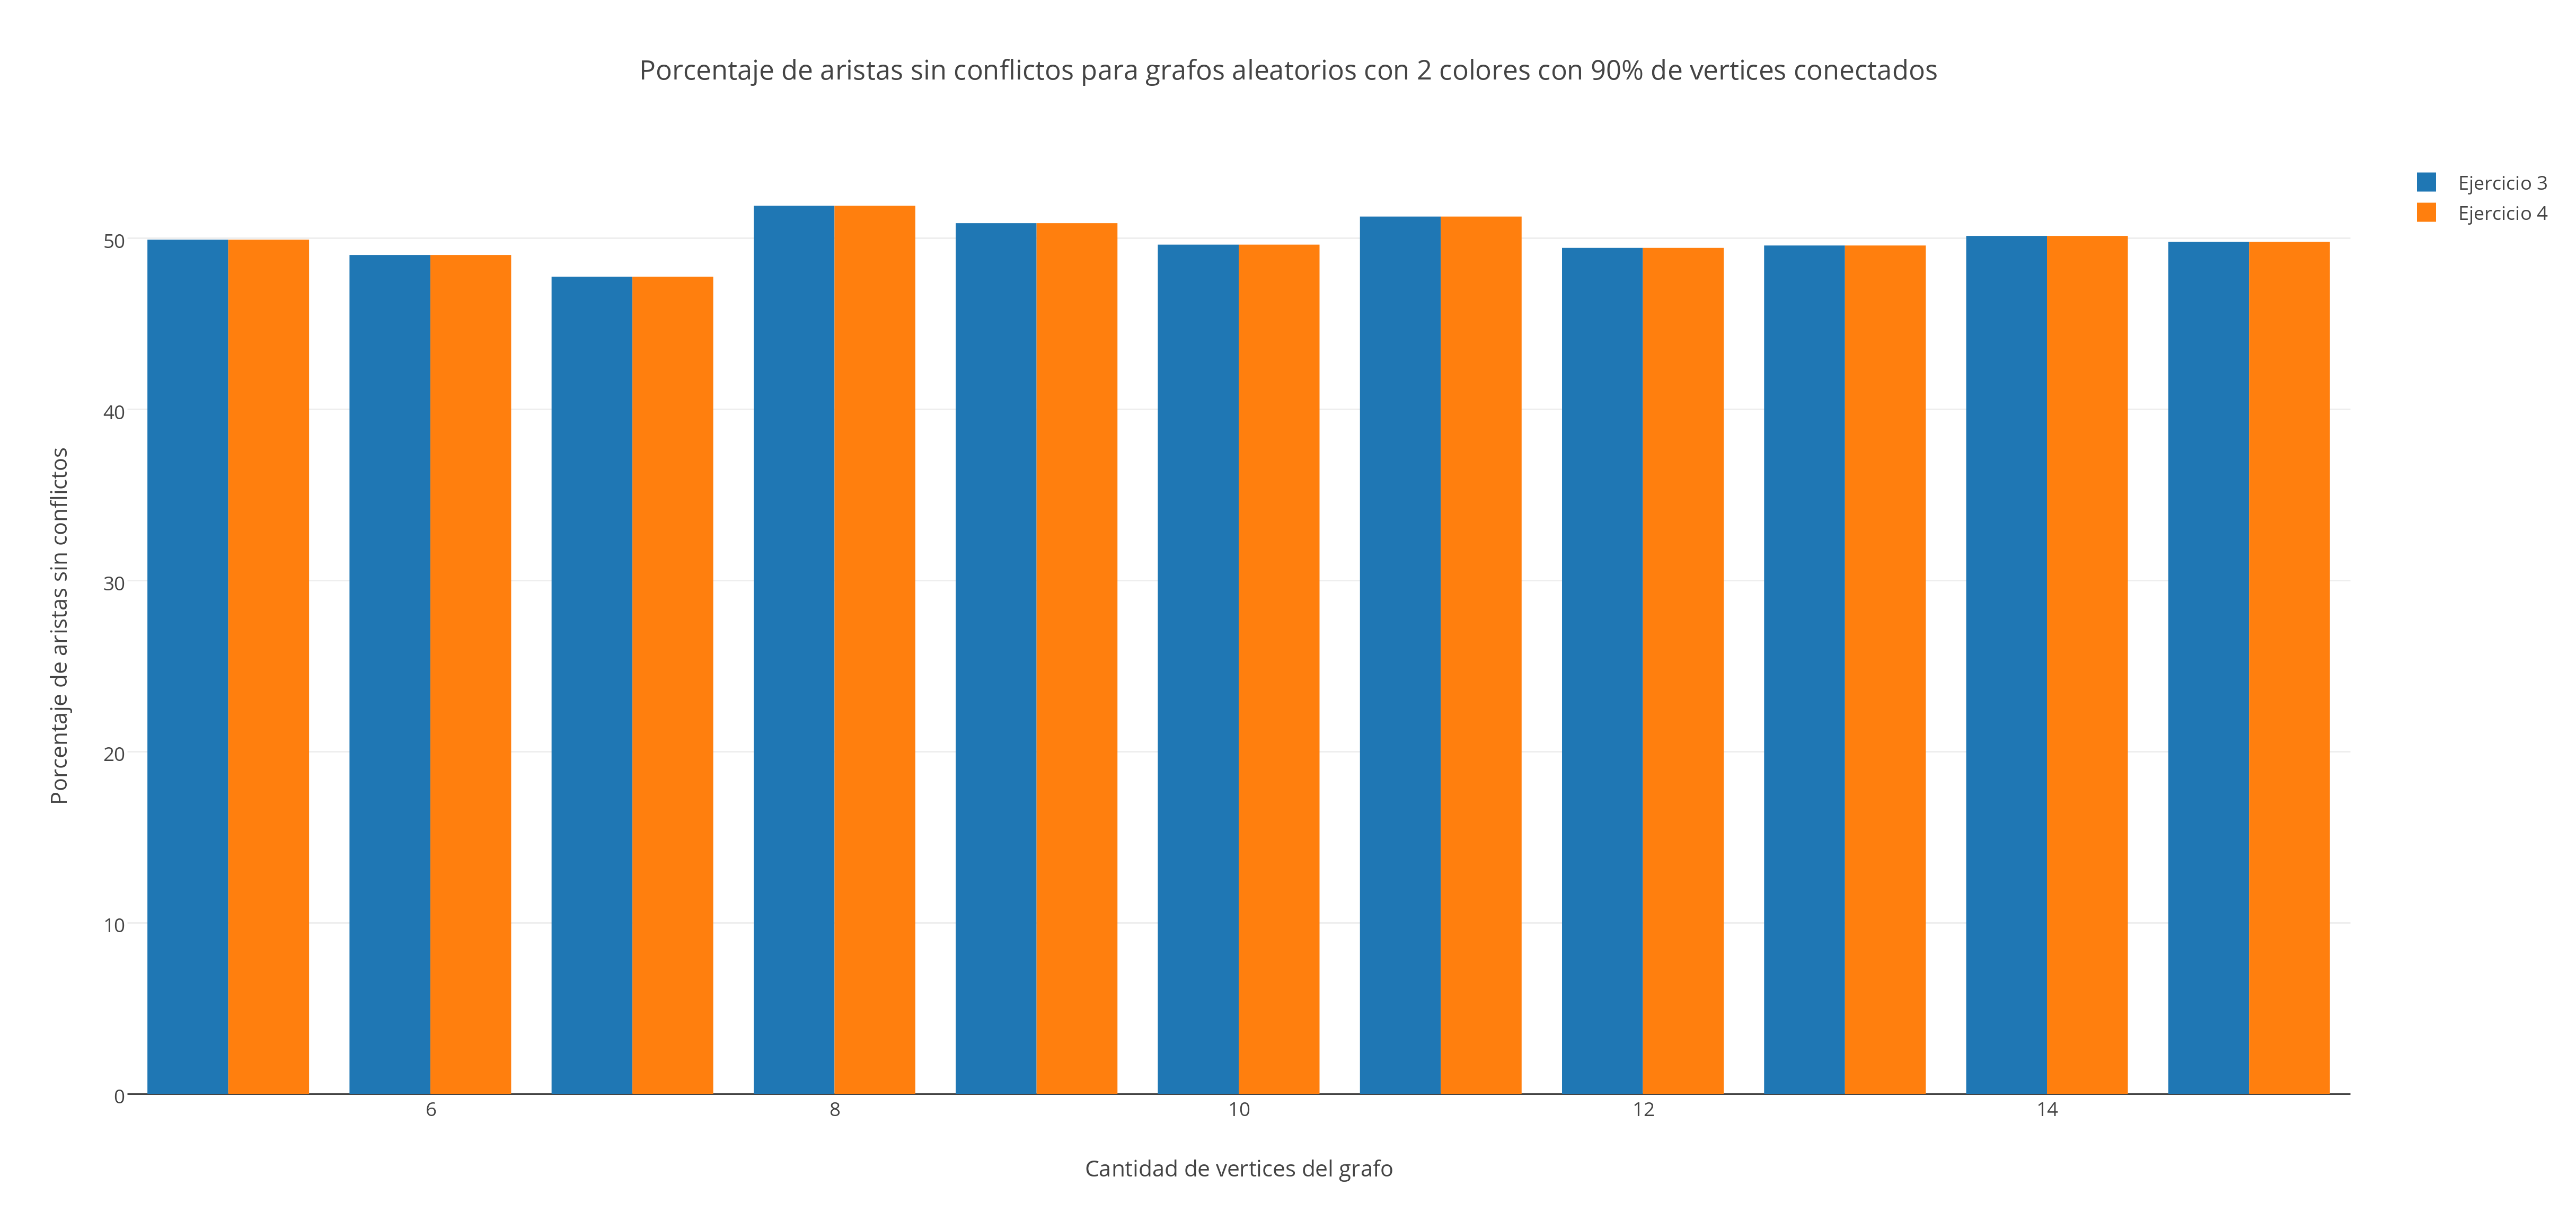
\includegraphics[scale=0.35]{./imagenes5/conf2.png}

Curiosamente, las calidades de solución son las mismas para los dos algoritmos. Lo que nos muestra que los algoritmos se comportan de manera muy similar para este caso. (Queda pendiente la demostración de este interesante hecho)\\
Esto nos lleva a la pregunta si se mantendrá esta similitud para los demás casos. Por lo tanto, aumentamos la cantidad de colores a 3, y aumentamos el rango de tamaño en los experimentos. \\

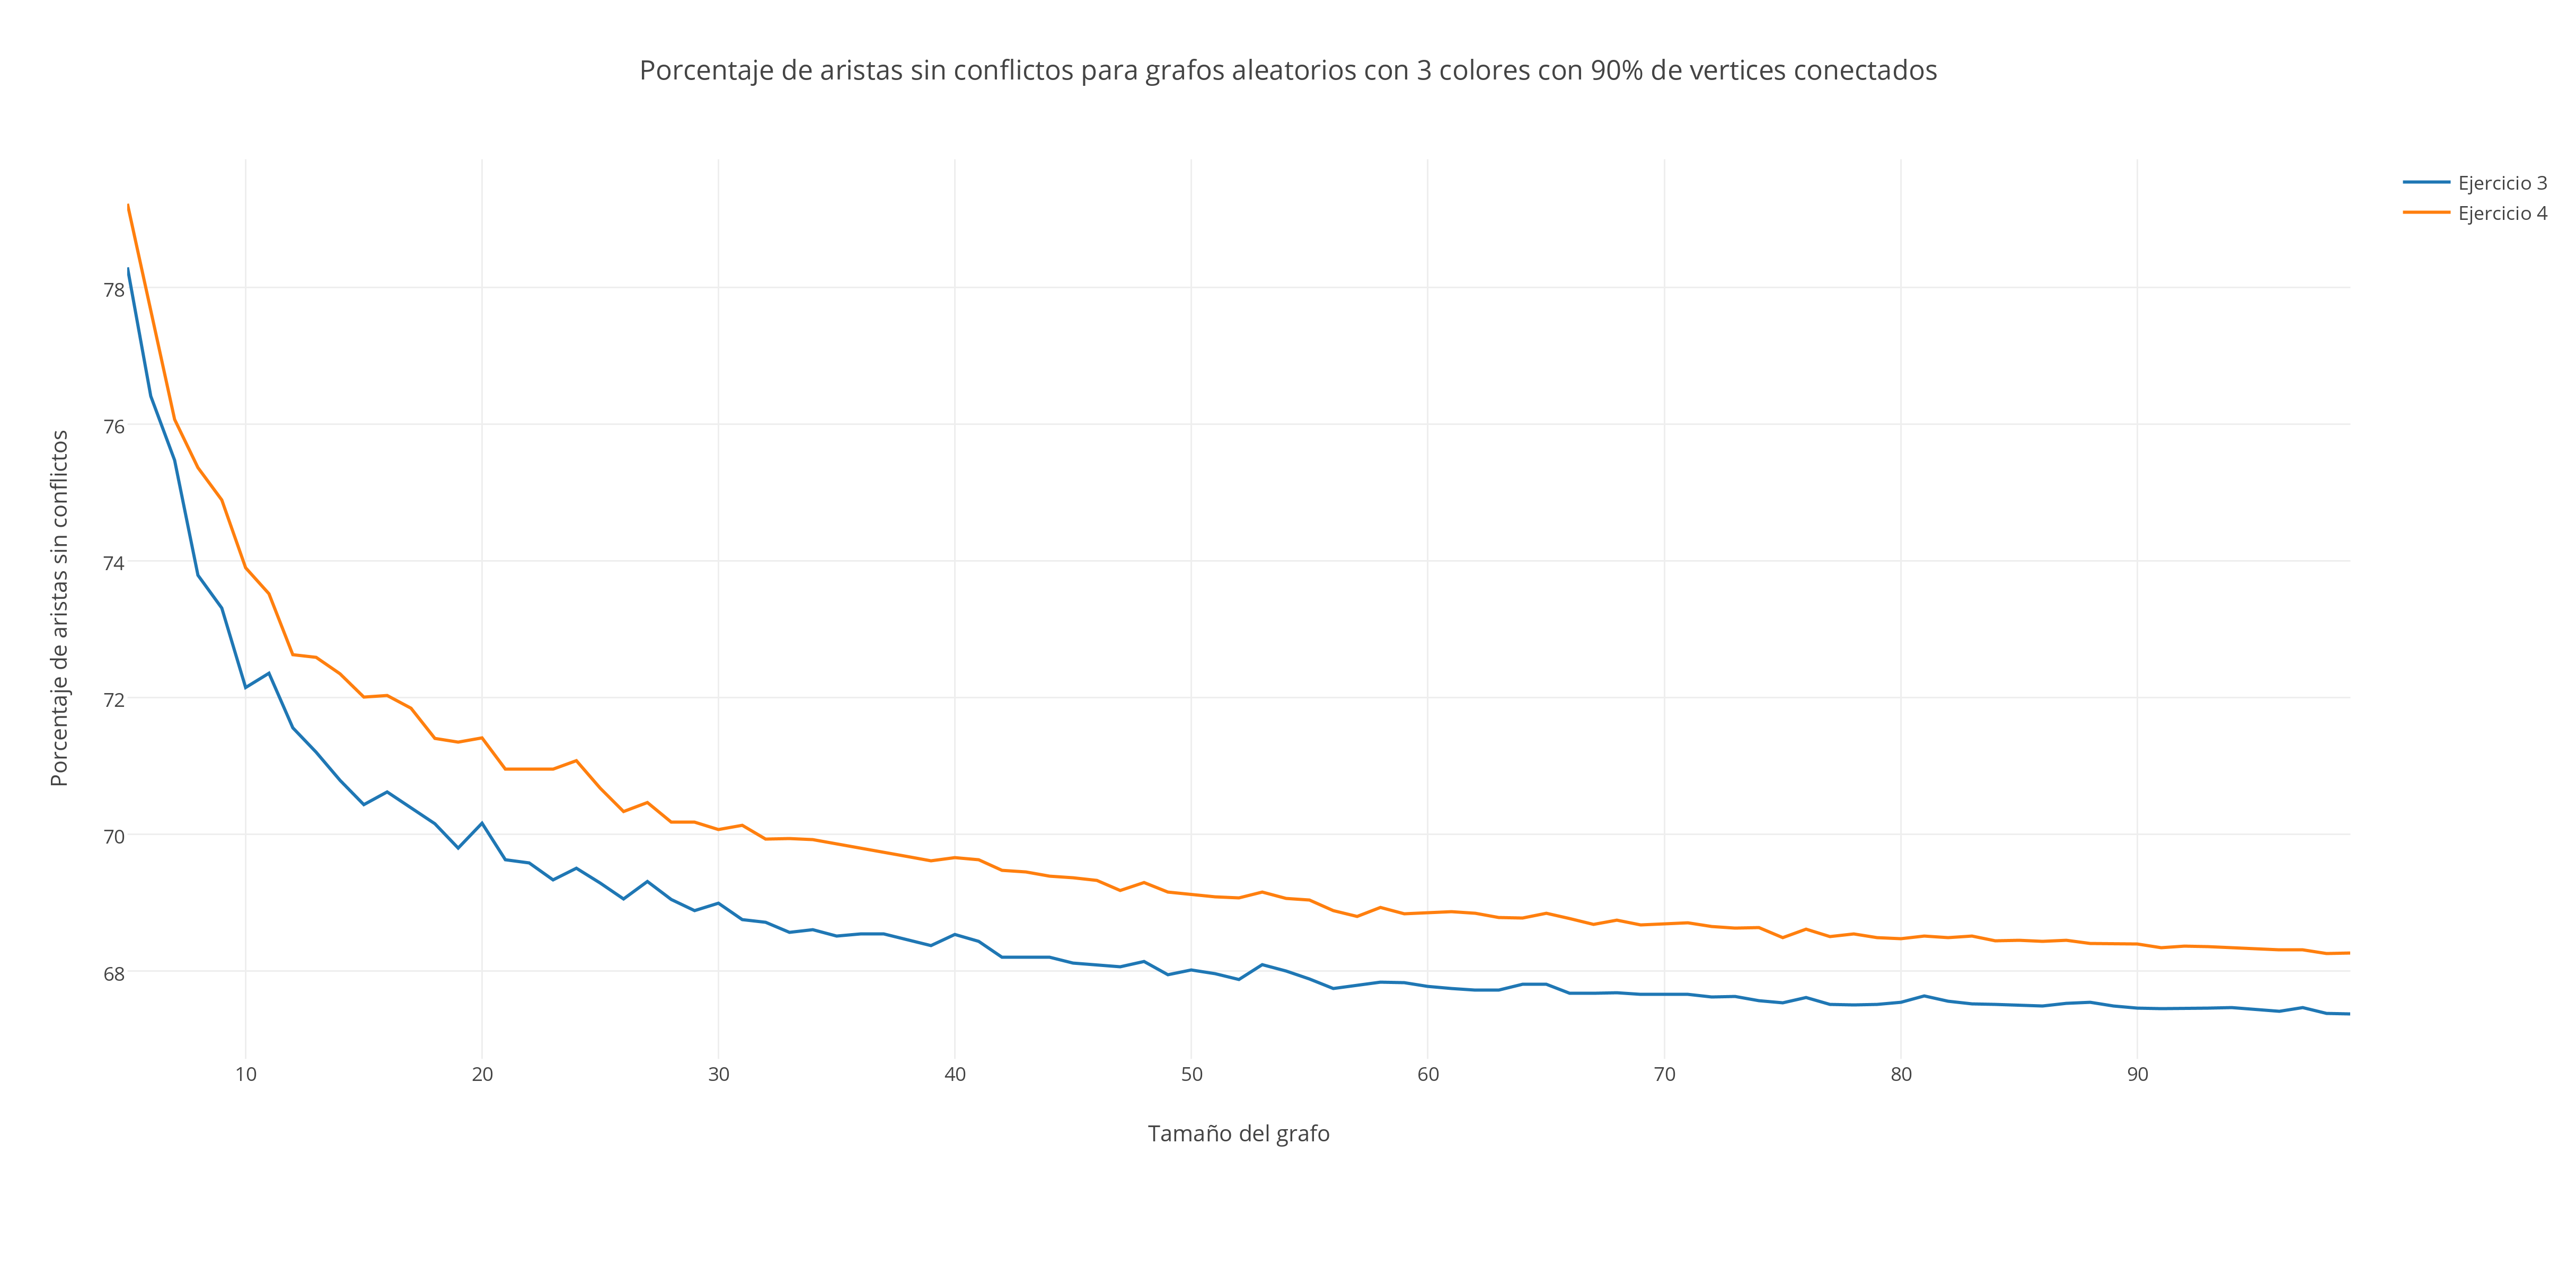
\includegraphics[scale=0.45]{./imagenes5/conf3.png}

Como podemos notar, las calidades ya empiezan a distinguirse entre los distintos algoritmos. Este caso da como ganador a la heuristica de busqueda local. \\

Realizamos un experimento más variando la cantidad de colores, pero siempre manteniendolos constante. La cantidad de colores elegidos fue de 10.\\

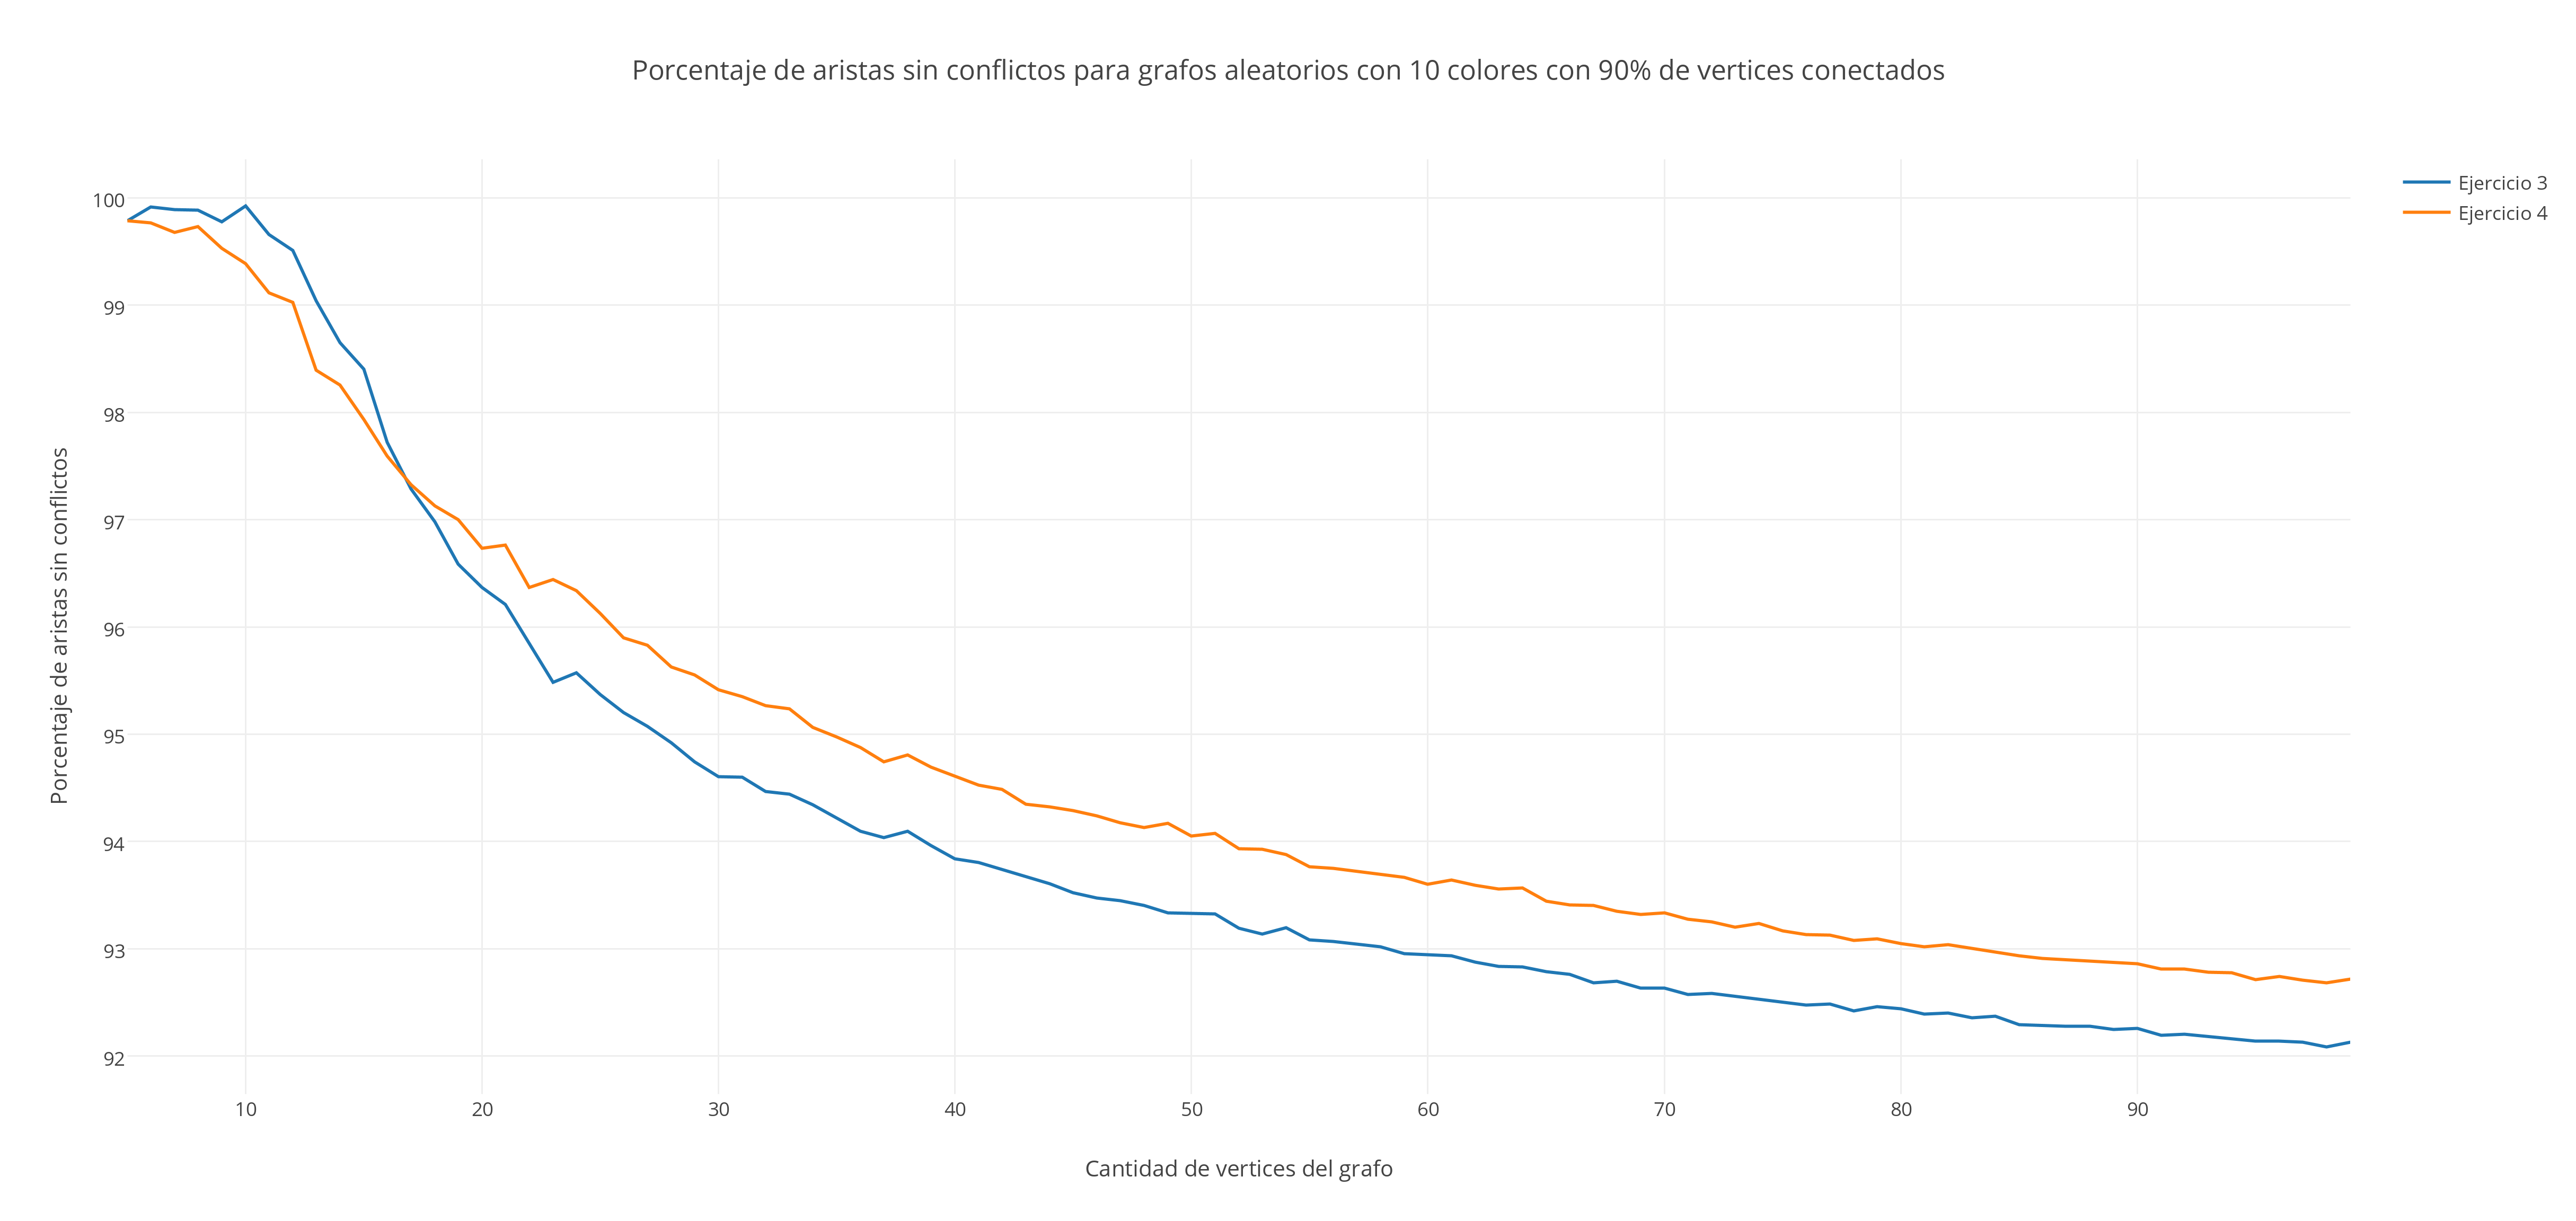
\includegraphics[scale=0.45]{./imagenes5/conf10.png}

Si bien con tamaños de grafo mas pequeños la heuristica golosa supera en calidad a la de busqueda local en calidad, luego de un aumento en el tamaño del grafo esta diferencia se revierte en favor del algoritmo del ejercicio 4. \\

Un dato interesante que no nos queda claro su por qué es el hecho de que en todos los experimentos con cantidad de colores fija $C$ pero con tamaño de grafo variable, la calidad se termina acercando al $100- \frac{100}{C}$ porciento. Por ejemplo, con $C=2$ estuvo alrededor del $50\%$, con $C=3$ alrededor del $66\%$, con $C=10$ alrededor del $90\%$. \\

Finalmente, decidimos probar con casos en los que la cantidad de colores aumenta linealmente con la cantidad de nodos del grafo. (Cada 4 vertices hay un nuevo color) \\

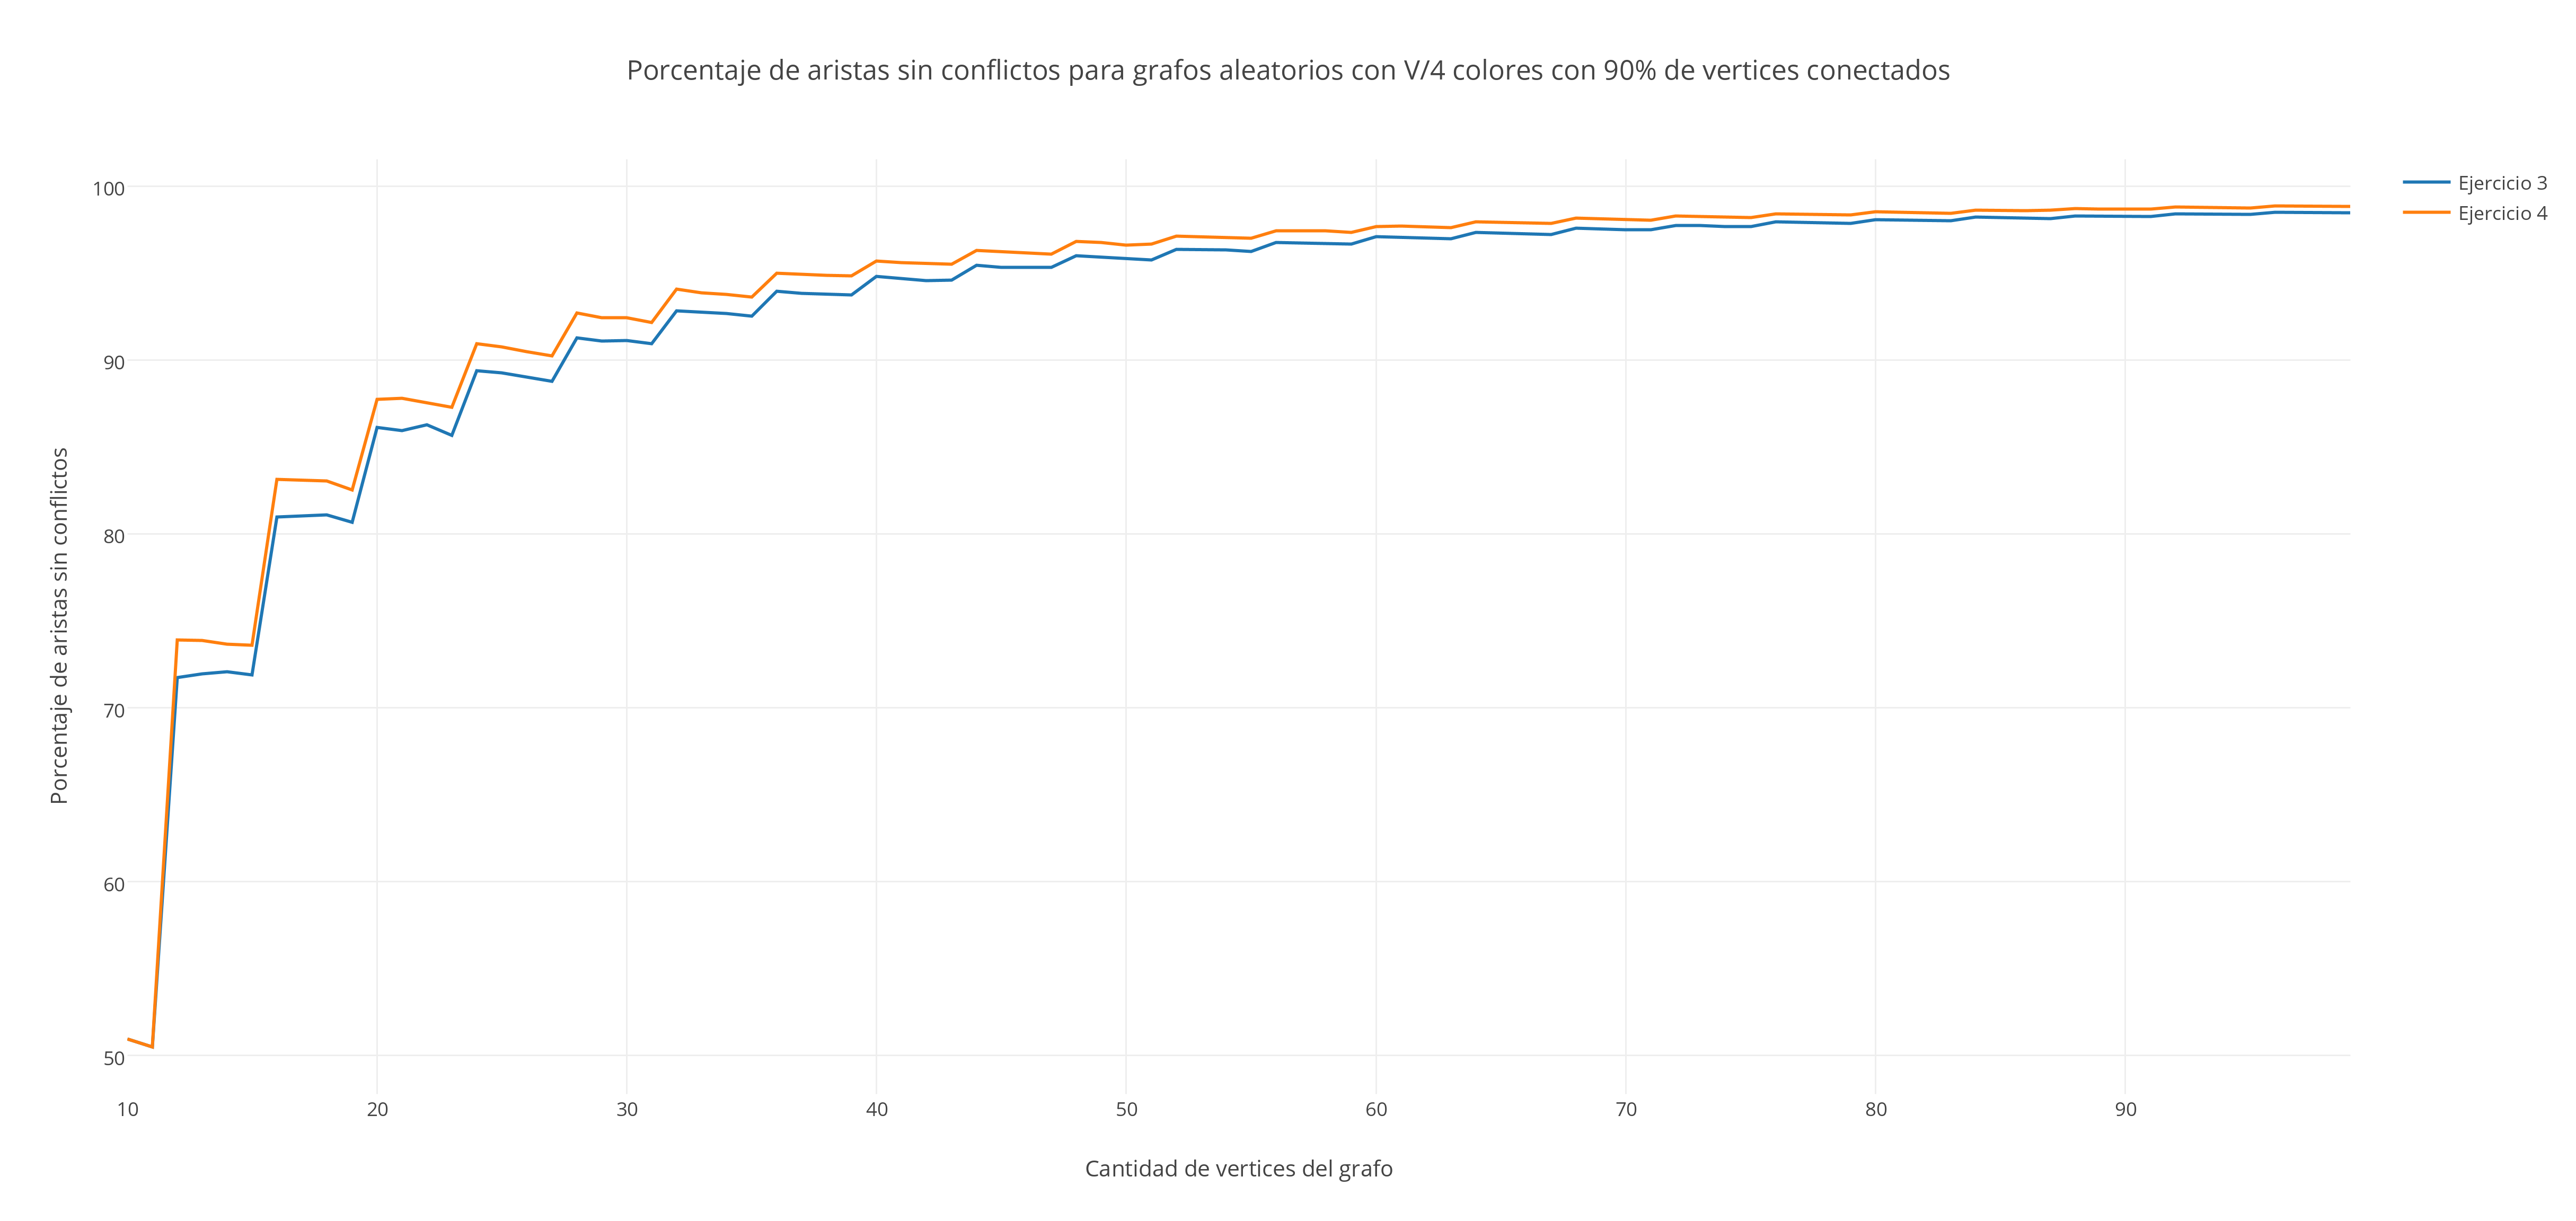
\includegraphics[scale=0.45]{./imagenes5/confv4.png}

Podemos notar al gráfico con saltos en los multiplos de cuatro, y esto es debido de que en esos casos los ejemplos pasan a tener un color más entre las opciones, por lo que el problema pasa a ser "más fácil" en general. \\
Esta comparación también da por ganadora a la heuristica de busqueda local. \\ \\

Resumiendo, pudimos notar en estos experimentos, que si bien en el analisis de calidad con grafos coloreables la heuristica del ejericicio 3 superó en calidad a la del 4, en los demás, esta última resultó ganadora. Creemos que los resultados del primer experimento se debieron a la poca cantidad de grafos analizados para analisis. \\

\subsection{Performance de solución}

En secciones anteriores las complejidades de cada algoritmo ya fueron estudiadas, y por lo tanto, se espera que los tiempos del algoritmo del ejercicio 3 sean notablemente menores que los del ejercicio 4.\\

En el siguiente gráfico se pueden comparar los tiempos de corrida para grafos de 2 colores en total.

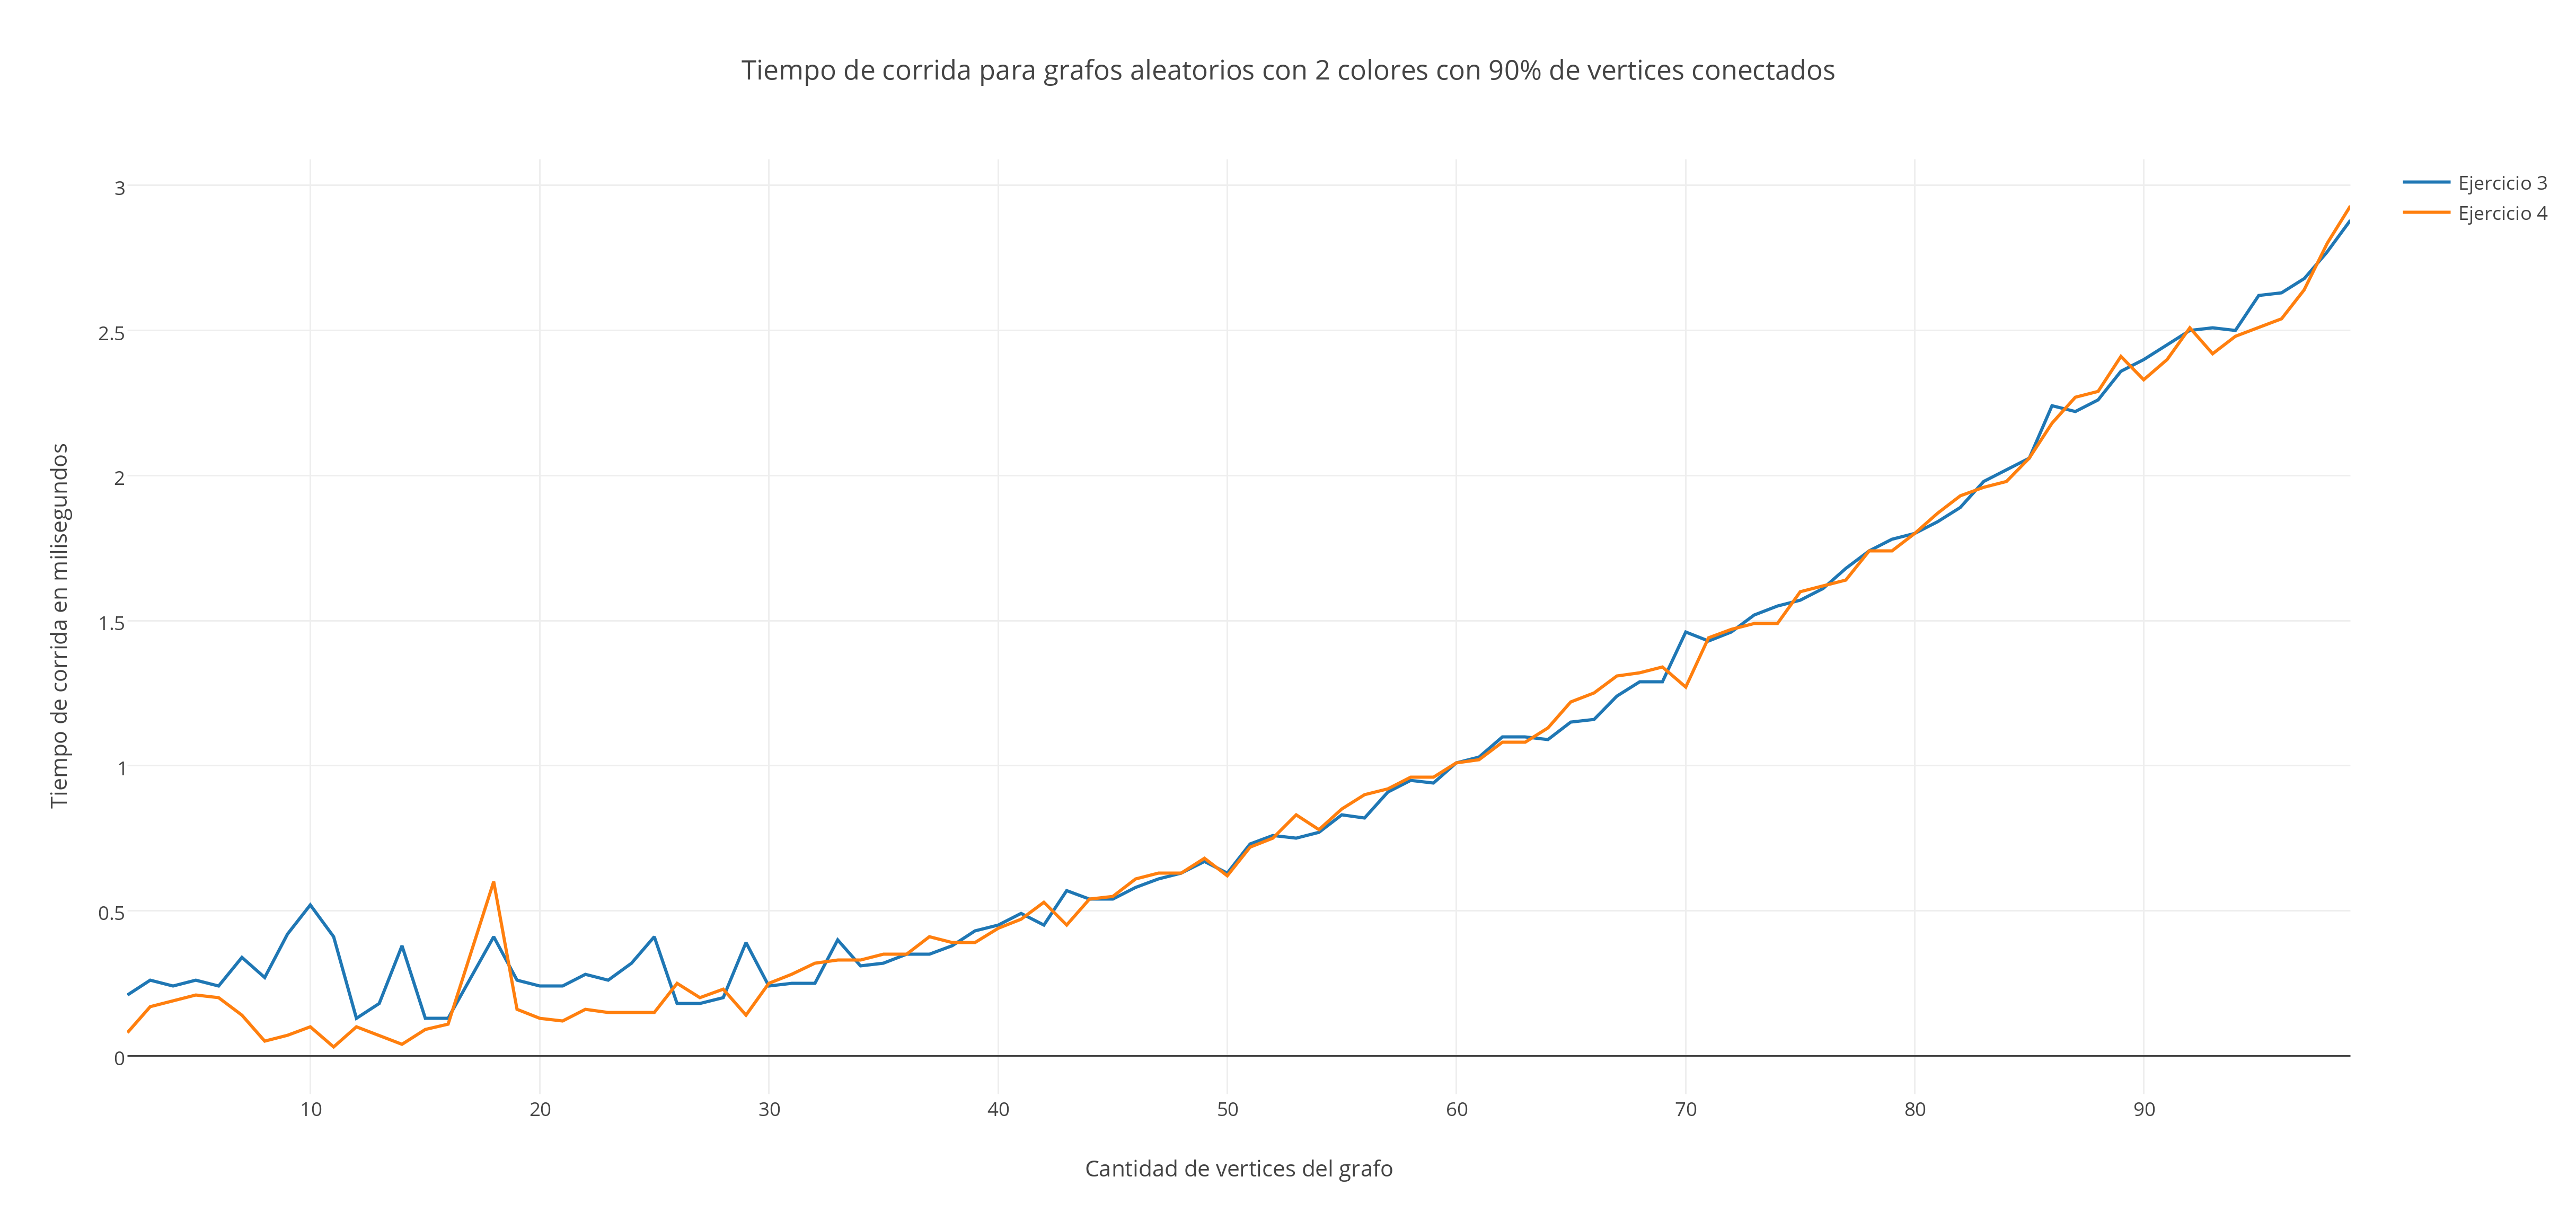
\includegraphics[scale=0.45]{./imagenes5/t2.png}

Los tiempos resultan muy parecidos, ya que el hecho de que haya pocos colores en total hace que no sea notorio el factor $C$ que tiene la complejidad del algoritmo del ejercicio 4. Por lo tanto, decidimos aumentar el la cantidad de colores, esta vez a $5$.

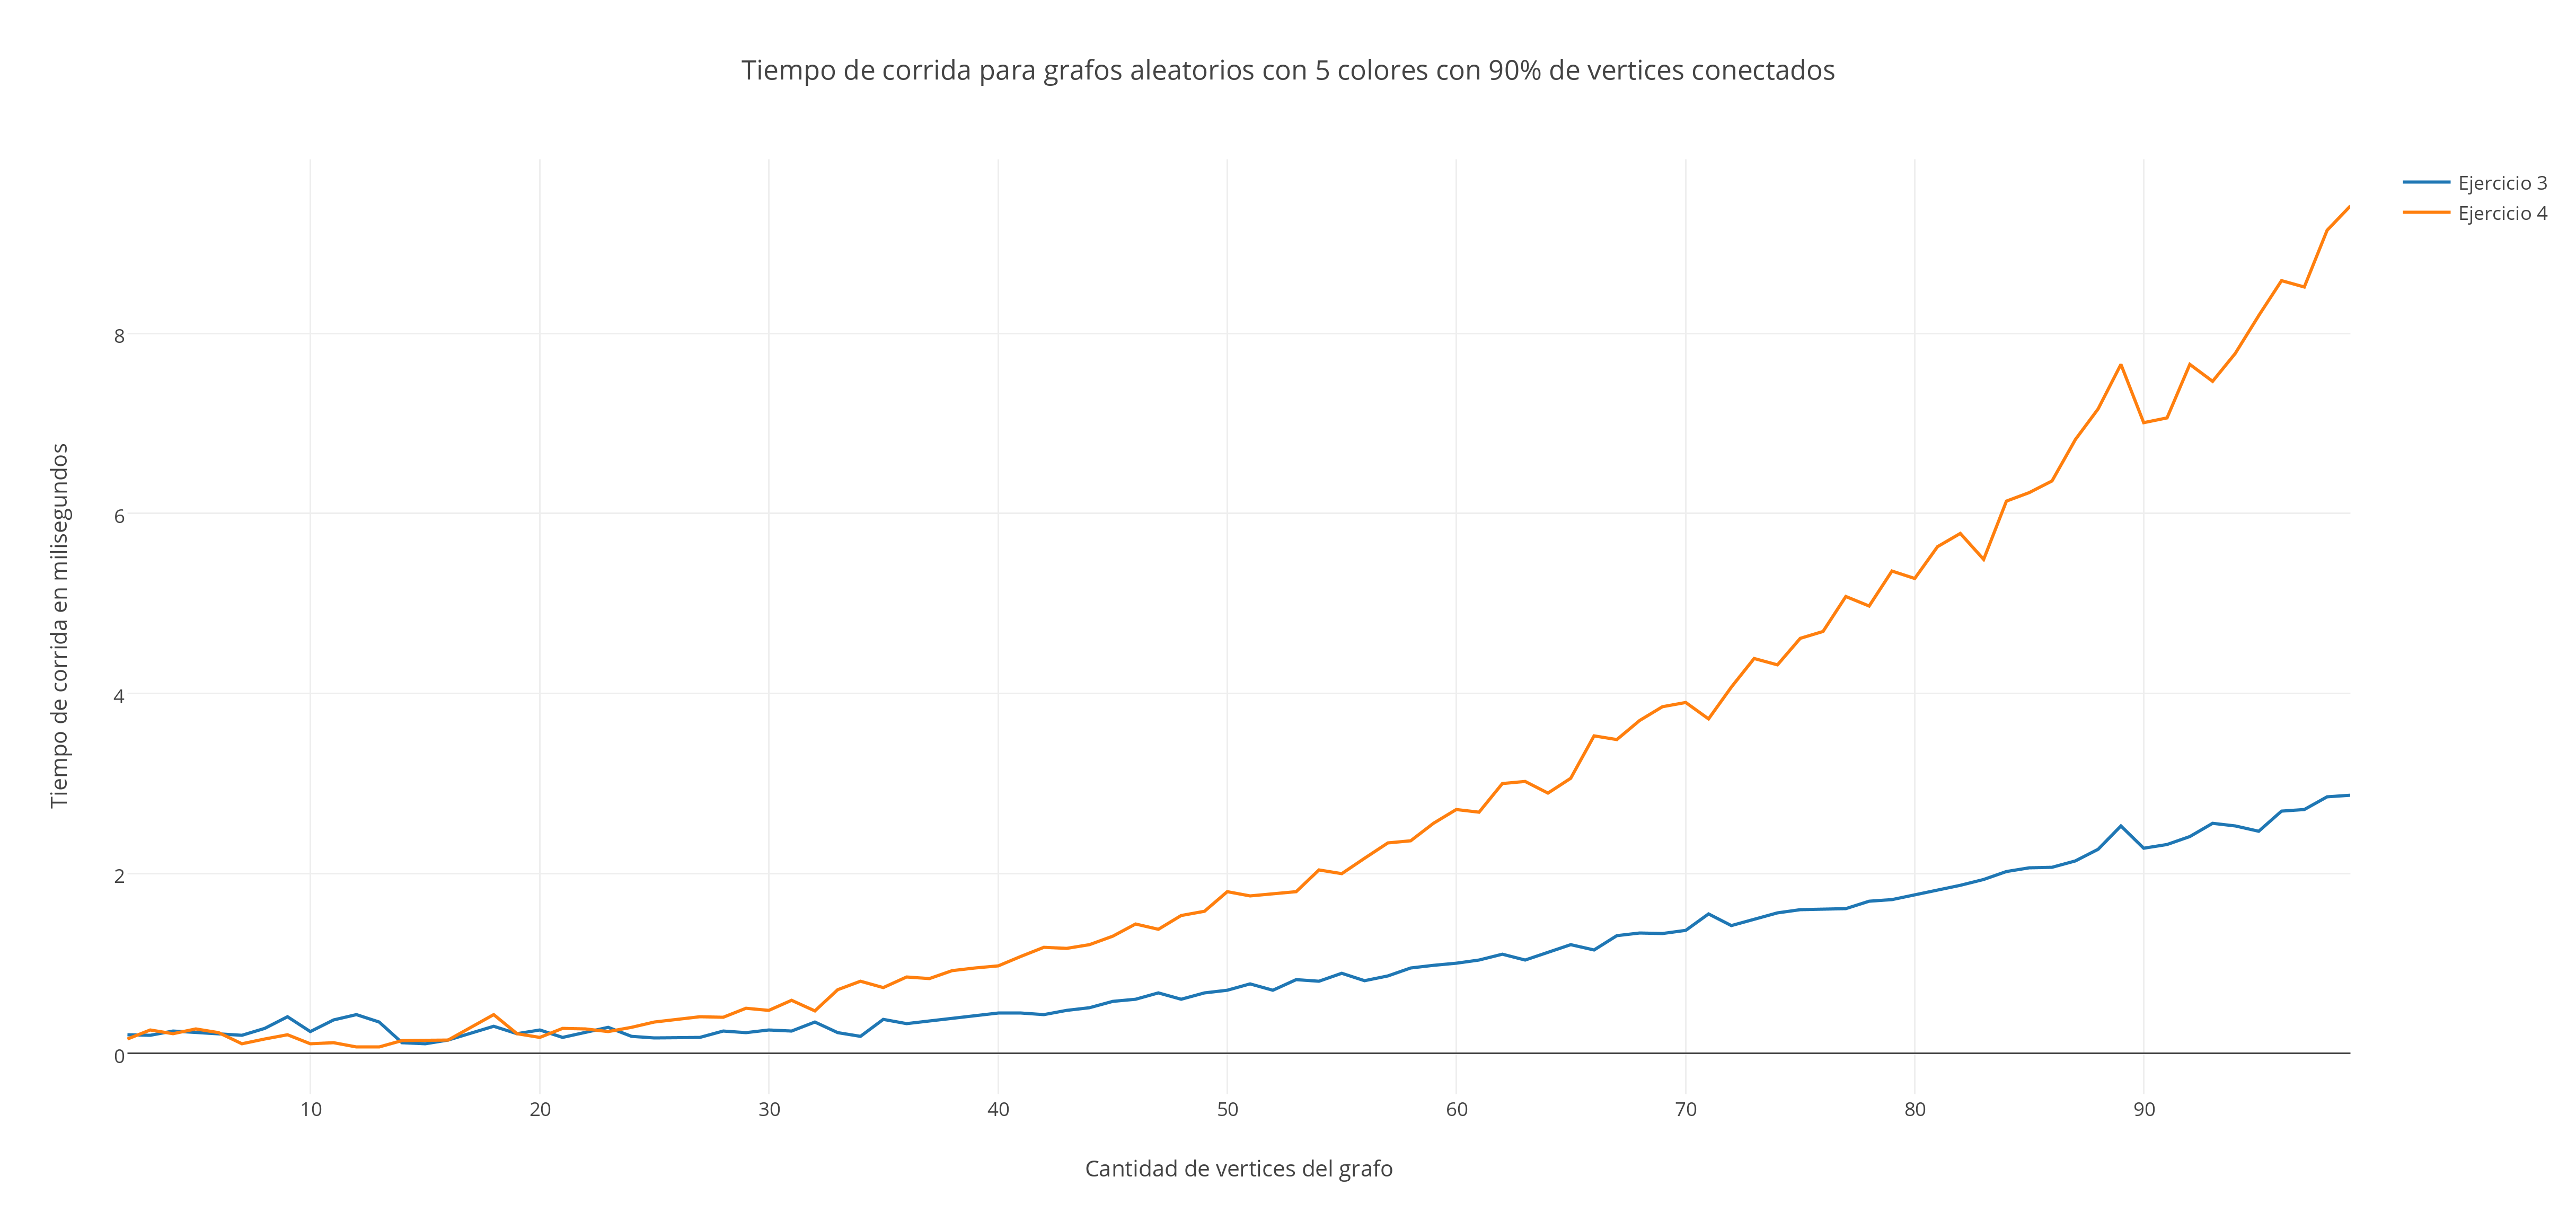
\includegraphics[scale=0.45]{./imagenes5/t5.png}

Y ahora la diferencia de tiempos resulta notoria, como habiamos conjeturado al principio de esta sección. \\


\subsection{Conclusión de comparaciónes}
Conluímos con que no hay un claro ganador entre los algoritmos, ya que ambos presentan un intercambio entre performance y calidad. \\
Por lo tanto, que algoritmo es mejor dependerá de nuestras necesidades, es decir, de nuestro contexto de uso. Por ejemplo, si nos interesan soluciones con la mayor calidad posible podemos optar por la implementación del ejercicio 4. Por el contrario, si lo que nos interesa es la velocidad, podremos optar por la implementacion del ejercicio 3. \\
Para este tipo de comparaciones, siempre se debe responder preguntas como ¿Qué tanta calidad se necesita? ¿Cuánta performance se puede perder? ¿Los casos que me interesan analisar resultan muy beneficiosos para el primer algoritmo o no hay mucha diferencia?








